\section{Results and discussion}


%%%%%%%%%%%%%%%%%%%%%%%%%%%%%%%%%%%%%%%%%%%%%%%%%%%%%%%%%%%%%
%%  Application to numerical simulations of BHVs under      %
%   quasistatic loading                                     %

\subsection{Numerical simulation of bioprosthetic heart valve deformation}
	
    Planar biaxial test simulations were conducted to ensure that $\Psi_{eff}$ (Eqn. \ref{c6:eqn:finalexponentialmodelformscaled}) and the elasticity tensor (Appendix \ref{sec:elasticitytensor}, Eqn. \ref{eqn:greenelasticityform}) were properly implemented in the finite element simulation framework.  We compared the computation time for both $\Psi_{eff}$ and Holzapfel-Gasser-Ogden model for biaxial simulation of bioprosthetic heart valve tissues and expectedly found no significant increase in computational cost. The total elapsed time for $\Psi_{eff}$ is 7.58 seconds in comparison to 6.40 seconds for the Holzapfel-Gasser-Ogden model, much faster than any micro-models can achieve.  

	Next we simulated tri-leaflet valves with model parameters derived from bovine pericardium, porcine aortic valve leaflet, and an idealized isotropic case. This is a simple demonstration of the use of the $\Psi_{eff}$ for the upscaling and homogenizing of micro-models. The model parameters for the bovine pericardium case were derived from the simplified structural model and model parameter of Aggarwal and Sacks \cite{aggarwal_inverse_2015}, and the resulting response matched very well qualitatively. Due to a lack of fiber mapping in the quasi-static simulation software used, some minor difference are still expected. We found no difficulty when simulating the pericardium, aortic, or isotropic valves. Suggesting that $\Psi_{eff}$ is quite robust numerically.
	
	
\begin{figure}
\centering
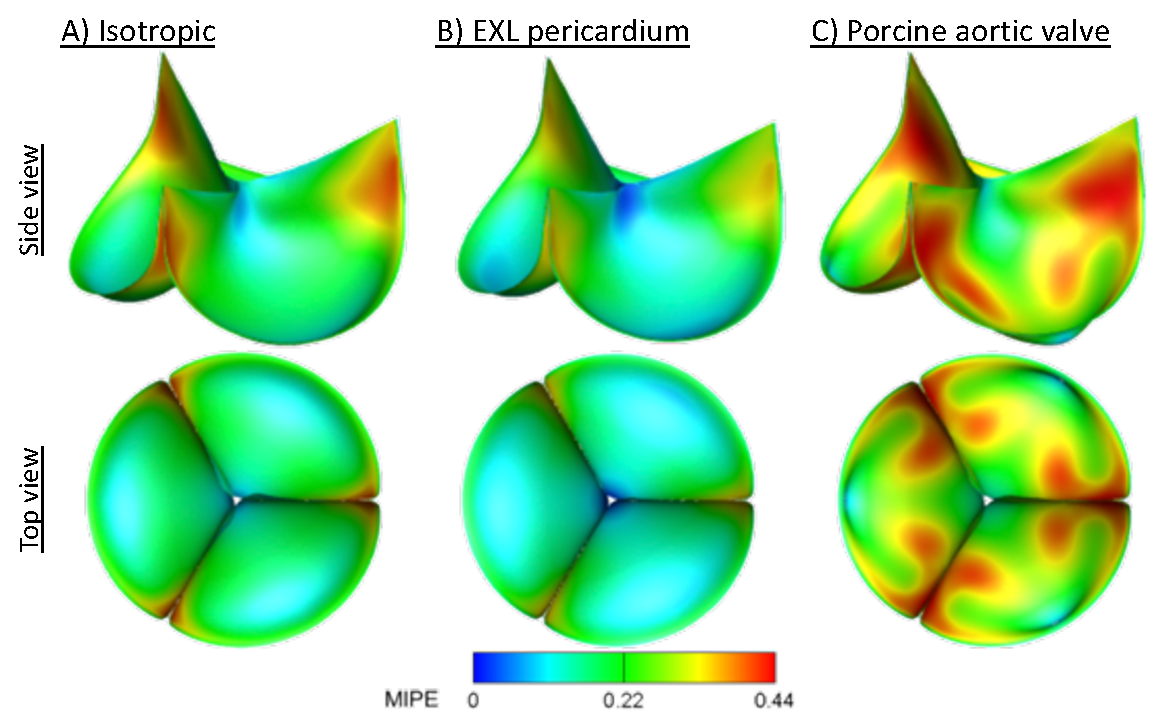
\includegraphics[width=\textwidth]{Images/chapter5/valvesimulations}
\caption{Simulations of intact tri-leaflet valves using A) the porcine aortic valve properties with an uniform fiber orientation distribution, B) exogenously cross-linked bovine pericardium properties with the most homogenous stress distribution, and C) the porcine aortic valve properties properties which results in a very heterogeneous stress distribution and the belly region caving in. The top row shows the side view of the valves at 80 mmHg and the bottom row shows the top-down view of the valves at the same transvalvular pressure.}
\label{fig:valvesimulations}
\end{figure}
    
    The material properties have significant effects on the mechanical behaviors of the leaflets (Fig. \ref{fig:valvesimulations}). The strain distributions within the leaflets were obtained for the pressure-loaded, fully-closed configurations of the valve, and then plotted with the maximum in plane Green-Lagrange strain (MIPE). When comparing the three different material, we can see that the native aortic valve properties result in significant heterogeneities in the deformation of the leaflets (Fig. \ref{fig:valvesimulations}C). Specifically, the belly region of the leaflets significantly protrudes out, increasing the load in the surrounding regions, especially near the commissures. This results in some stress concentrations that are not conducive to heart valve durability and health in general. The bovine pericardium valve (Fig. \ref{fig:valvesimulations}B) and the isotropic valve (Fig. \ref{fig:valvesimulations}A) on the other hand have significantly more homogeneous leaflet deformations, especially from the top-down view. Both of these undergo approximately the same deformation of 0.2 in MIPE. The largest difference between the two is near the commissure regions of the valve. Where the isotropic case is under significantly higher strain. Functionally, the material properties of the exogenously cross-linked bovine pericardium are the most suitable for heart valve leaflets, which distributes the stresses more evenly. 
    
    Much of the reasons behind these differences are likely to be due to the differences between the apparent mechanical properties \textit{in vivo} and the measured mechanical response in the laboratory setting. This is especially true for the aortic valve, which is extremely anisotropic with very high compliance in the radial direction of the leaflets. This difference is most likely due to the mismatch of referential configuration between the two states. Residual strain or residual stress has significant impact on the functional properties of the leaflets, specifically the apparent anisotropy and stiffness. Collagen fiber directions and varying regional properties can also have significant impact on the functional properties of the leaflets, and thus the results of the simulation. The valve leaflet shape, root geometry and properties, the arterial or ventricular geometry and loading conditions, can all be significant factors affecting the functions and stress distribution of the valve leaflets. Furthermore, how these factors affect the fluid dynamics of the valves is also an interesting question, suitable for further study. All in all, this is meant to be a demonstration and proof of concept for using $\Psi_{eff}$ to handle a wide range of soft tissue behaviors and anisotropy for the simulation of biological organs, in this case heart valves. Further and more detailed studies will be reserved for the future.  



\subsection{Permanent set simulation of bioprosthetic heart valve}
    This initial was done with 1) homogenous material parameters simular to bovine pericardium from Sacks and Zhang \cite{sacks_novel_2016}, 2) the Edward valve geometry from \cite{aggarwal_inverse_2015}, and collagen fiber distributions aligned with the circumference direction and a standard deviation of $30^\circ$. The key result is that permanent set slow done after around 20 million cycles and nearly completely seizes after 30 million cycles (Fig. \ref{c6:fig:psdeformation} \&\ref{c6:fig:psnoi}). This effect is closely linked the microstructural of the collagen fiber network. The gradual slow down is correlated with the straightening and recruitment of collagen fibers. This was predicted from the constitutive model (Eqn. \ref{c6:eq:fullEXLmodel}) (Fig. \ref{fig:parametric}). This is an important structural response, which allows us to predict the final reference geometry of the BHV. Since 30 million cycles corresponds to only 1 year after being surgically implanted, the BHV will remain in this configuration for the rest of its 9-14 year life span. By optimizing the initial BHV design so that the peak stress is minimal in the configuration after permanent set has seized, we can potentially improve the durability of BHVs by minimizing the load on the collagen fibers. Because collagen fibers have high rates of failure after being extended by 7-8\% \cite{lanir_structural_1979}\cite{buehler_atomistic_2006}, more evenly distributing the stresses can reduce this mode of failure. 
    
%%%%%%%%%%%%%%%%%%%%%%%%%%%%%%%%%%%%%%%%%%%%%%%%%%%%%%%%%%%%
%-------------------	begin FIGURE 	-------------------%
\begin{figure}
\centering
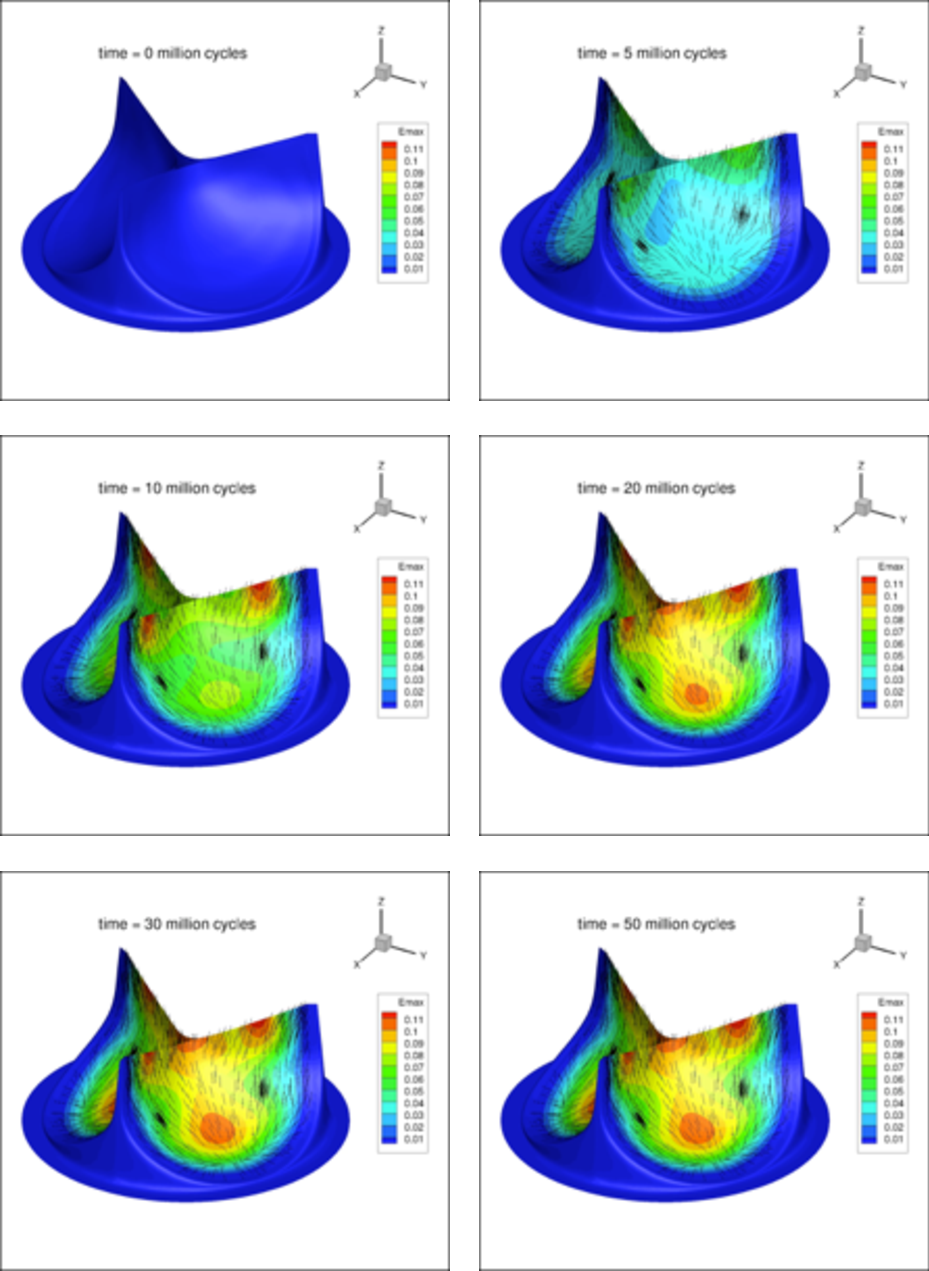
\includegraphics[width=5in]{Images/chapter6/psdeformation.pdf}
\caption{The simulation of the evolution of the referential configuration with the maximum principal in\Hyphdash plane Green-Lagrange strain (MIPE) overlayed on top at different cycle levels. Colors indicate the magnitude of MIPE, and the lines indicate the principal direction of the permanent set deformation.}
\label{c6:fig:psdeformation}
\end{figure}
%-------------------	 end FIGURE 	-------------------%
%%%%%%%%%%%%%%%%%%%%%%%%%%%%%%%%%%%%%%%%%%%%%%%%%%%%%%%%%%%%

%%%%%%%%%%%%%%%%%%%%%%%%%%%%%%%%%%%%%%%%%%%%%%%%%%%%%%%%%%%%
%-------------------	begin FIGURE 	-------------------%
\begin{figure}
\centering
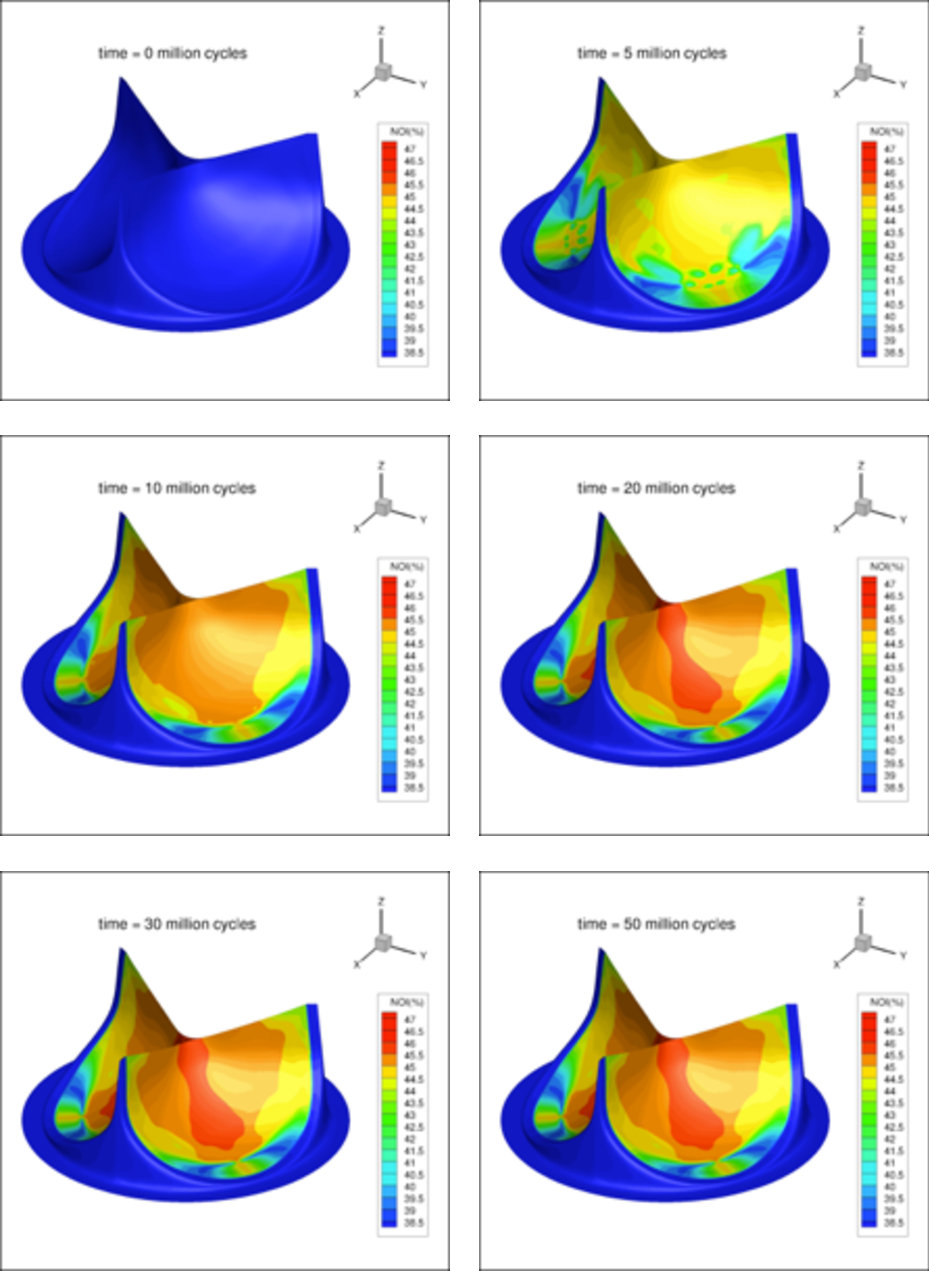
\includegraphics[width=5in]{Images/chapter6/permanentsetnoi.pdf}
\caption{The simulation of the evolution of the referential configuration with the normalized orientation index (NOI) overlayed, showing the changes in the degree of alignment of collagen fibers at different cycle levels. Higher NOI indicate higher aligned fiber orientation distributions.}
\label{c6:fig:psnoi}
\end{figure}
%-------------------	 end FIGURE 	-------------------%
%%%%%%%%%%%%%%%%%%%%%%%%%%%%%%%%%%%%%%%%%%%%%%%%%%%%%%%%%%%%
    
    Here we also note that the regions that undergo most permanent set are: the belly region, center of the free edge, and the regions near the commissures, where the leaflets initial makes contact (Fig. \ref{c6:fig:psdeformation}). These regions are also the most common regions of failure in BHVs. Due to the change in reference configuration, the collagen fibers in these regions recruit more quickly and may even held in a constant extended state. This can have dramatic consequences on the likelihood of failure of these collagen fibers due to their low extensibility, and could be a major mechanism for the fiber level damage in BHVs. 
    
    
    We have also shown that we can predict the change in the collagen fiber architecture (Fig. \ref{c6:fig:psnoi}). Here we plotted the normalized orientation index (NOI)
    \begin{equation}
        NOI = \frac{\sigma_iso - \sigma(s)}{\sigma_iso},
    \end{equation}
    which is based on how spread apart (standard deviation $\sigma$) is collagen fiber orientation is. Here, $NOI = 1$ indicate fully aligned distributions (delta distributions), which $NOI = 0$ indication that the fiber distribution is an uniform distribution. We can see that the belly region and the free edge undergoes the greatest degree of realignment. This is most likely due to the fact that these two regions receives the least amount of support from the neighboring leaflets. The most important aspect of being able to predict the structural changes is that we can use it to compute the degree of recruitment of collagen fibers in a similar method to chapter \ref{c2:sec:233}. This allows us to compute the distribution of collagen fiber by their stretches after being straightened. This mechanism can be used to potentially develop a strain-level dependent model for the likelihood of collagen fiber damage in a future extension. 

    
